 \section{Javassist}

\subsection{Javassist}

\subsubsection{Introduction}

\textbf{Javassist is a class library for editing Java bytecode and enabling:}

\begin{itemize}
	\item class modification at load time (load-time MOP);
	\item creation of a new class at run time.
\end{itemize}

\textbf{t is a high-level API, it does not require knowledge of bytecode specifications}

\begin{itemize}
	\item 100 Java, portable (JVM 1.2+, compliant Java 11)
	\item it is based on the class loading model
\end{itemize}

\textbf{Javassist is a largely used software}

\begin{itemize}
	\item it is part of the jBoss architecture (Red Hat)
	\item it has been developed by Shigeru Chiba
\end{itemize}

\subsubsection{Javassist General Architecture}

\begin{center}
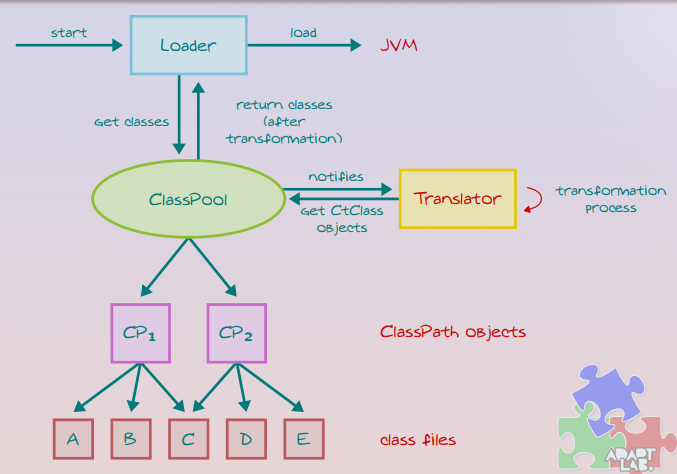
\includegraphics[scale=0.3]{15-javassist}
\end{center}

\subsubsection{Javassist Core API}

High-level API: source code abstractions

Improvement over Java structural reflection through a parallel reification of Java classes and primitive types:

\begin{itemize}
	\item CtClass, CtMethod, CtConstructor, CtField,
	\item FieldInitializer, CtPrimitiveType, Modifier . . .
\end{itemize}

Introduction of new classes to decompose the class loading process and enabling class modification (at load time):

\begin{itemize}
	\item Loader, ClassPool, ClassPath
	\item Translator.
\end{itemize}

\subsubsection{ClassPool and Translator}

\textbf{ClassPool}

A container of CtClass objects. Every loaded class passes through this object.

\begin{itemize}
	\item get(String): returns a reference to a CtClass;
	\item toClass(): translates a CtClass into a standard class format;
	\item insertClassPath, appendClassPath: manage class lookup process
	\item make*: create classes, interfaces from scratch;
	\item static services to get the class pool with or without Translator
\end{itemize}

\textbf{Translator}
An observer of Loader. This interface should be implemented to translate a class file when the class file is loaded into the JVM.

\begin{itemize}
	\item start(ClassPool): translator initialization;
	\item onLoad(ClassPool, String): before the class is given to the loader minus the time for modifications.
\end{itemize}

\subsubsection{CtClass vs Class}

Provides the protocols for operating on a class (before it is loaded into the JVM) or for dynamic creation of new classes.

\textbf{Introspection}

\begin{itemize}
	\item same as java.lang.reflect;
	\item isModified, isFrozen (already loaded, cannot be modified).
\end{itemize}

\textbf{Intercession}

\begin{itemize}
	\item setName, setSuperclass, setModifiers, . . . ;
	\item addInterface, addField, addMethod, . . . ;
	\item replaceClassName: replaces classname occurrences within a class (using a map).
\end{itemize}

\textbf{Transformation}

\begin{itemize}
	\item getClassFile: returns a ClassFile object (javassist.bytecode), for low-level bytecode manipulation;
	\item instrument(CodeConverter): applies a code converter on methods and constructors
\end{itemize}

\subsubsection{CodeConverter}

Instances of this class specifies how to instrument the bytecodes representing a method body.

\begin{itemize}
	\item They are passed to CtClass.instrument() or CtMethod.instrument() as a parameter.
\end{itemize}

High-level modifications inside method bodies enables to:

\begin{itemize}
	\item insert a call to the method m before or after another method call
	\item redirect a method call to another method m
	\item redirecting a field access to another field f
	\item replace a field access by a static method call
	\item replace a new statement by a static method call.
\end{itemize}

\subsubsection{Example: Binary Component Adaptation}

Update classes so that they fit into a framework, transforming their bytecode automatically.

We have a class Calendar implementing a third-party Writable interface:

\begin{lstlisting}[language=Java]
class Calendar implements Writable {
	public void write(PrintStream s) { ... }
}
\end{lstlisting}

\textbf{In a new version of the class library, Writable has been replaced by Printable (it also defines print()): we have to update Calendar.}

\begin{lstlisting}[language=Java]
class Calendar implements Printable {
	public void write(PrintStream s) {...}
	public void print() { this.write(System.out); }
}
\end{lstlisting}

\subsubsection{Example: Binary Component Adaptation (Cont’d)}

\begin{lstlisting}[language=Java]
import java.io.PrintStream ;
class Exemplar implements Printable {
	public void write(PrintStream s) { ... }
	public void print() { write(System.out); }
}
\end{lstlisting}

\begin{lstlisting}[language=Java]
import javassist.ClassPool;
import javassist.Loader;
public class RunAdaptation {
	public static void main(String[] args) {
		Adapter adapter = new Adapter();
		ClassPool pool = ClassPool.getDefault();
		Loader loader = new Loader(pool);
		loader.addTranslator(pool, adapter);
		loader.run("TestApp", args);
	}
}
\end{lstlisting}

\begin{lstlisting}[language=Java]
import javassist.* ;
class Adapter implements Translator {
	CtMethod printM; CtClass printable;
	public void start(ClassPool p) {
		printable = p.get("Printable");
		CtClass ex = p.get("Exemplar");
		printM=ex.getDeclaredMethod("print",null);
	}
	public void onLoad(ClassPool p, String cn) {
		CtClass cls = p.get(cn);
		CtClass[] interfaces = cls.getInterfaces();
		for (int i=0; i<interfaces.length; i++) {
			if (interfaces[i].getName()
						.equals("Writable")) {
				interfaces[i] = printable;
				cls.setInterfaces(interfaces);
				cls.addMethod(
					CtNewMethod.copy(printM, cls, null));
				return;
			}
		}
	}
}
\end{lstlisting}

\subsubsection{Javassist Bytecode-Level API}

\begin{itemize}
	\item low-level API: bytecode abstractions;
	\item core API services are implemented with it;
	\item can be used for finer-grained transformations:
	\item ClassFile is the base entity for bytecode editing;
	- ClassFile = < ConstPool, Methods, Fields, Attributes>;
	- obtained from CtClass, stream or from scratch;
	- write to output stream;
	\item – OpCode defines all bytecode instructions as constants
	- ALOAD, ASTORE, INVOKESPECIAL, . . .
\end{itemize}

\subsubsection{ClassFile}

\textbf{Intercession}

\begin{itemize}
	\item addAttribute(AttributeInfo);
	\item addMethod(MethodInfo);
	\item addField(FieldInfo);
	\item renameClass, setName;
	\item setAccessFlag, setInterfaces, setSuperclass.
\end{itemize}

\textbf{Introspection}

\begin{itemize}
	\item getConstPool, getAttribute, getMethod, . . . ;
	\item isFinal, isAbstract, isInterface.
\end{itemize}

\subsubsection{XXXInfo (MethodInfo, FieldInfo, ...)}

\textbf{All XXXInfo classes enable introspection and intercession}

– e.g., MethodInfo has getCodeAttribute().

\textbf{CodeAttribute is a structure with raw bytecode:}

– (byte[]) + info (length, max stack, exceptions, . . . )

\textbf{CodeIterator is used to parse and manipulate raw code:}

– insert code, replace code, . . . ;
– go to next instruction . . .

\subsubsection{Example: How to Simulate the Meta-Object Approach}

\begin{lstlisting}[language=Java]
package sample.reflect;
import javassist.tools.reflect.Metalevel;
import javassist.tools.reflect.Metaobject;
public class Person {
	public String name;
	public static int birth = 3;
	public Person(String name, int birthYear) { this.name = name; birth = birthYear; }
	public String getName() { return name; }
	public int getAge(int year) { return year - birth; }
	public static void main(String[] args) {
		Person p = new Person( args[0], 1948 );
		System.out.println("name: " + p.getName());
		System.out.println("object: " + p.toString());
		// change the metaobject of p.
		if (p instanceof Metalevel) {
			((Metalevel)p)._setMetaobject(new Metaobject(p, null));
			System.out.println("«the metaobject was 	changed.»");
		}
		System.out.println("age: " + p.getAge(2018));
	}
}
\end{lstlisting}

\begin{lstlisting}[language=Java]
[16:38]cazzola@hymir:~/tsp> java sample.reflect.Person "Gladstone Gander"
name: Gladstone Gander
object: sample.reflect.Person@34033bd0
age: 70
\end{lstlisting}

\subsubsection{Example: How to Simulate the Meta-Object Approach (Cont’d)}